\documentclass[14pt]{extbook}
\usepackage{multicol, enumerate, enumitem, hyperref, color, soul, setspace, parskip, fancyhdr} %General Packages
\usepackage{amssymb, amsthm, amsmath, latexsym, units, mathtools} %Math Packages
\everymath{\displaystyle} %All math in Display Style
% Packages with additional options
\usepackage[headsep=0.5cm,headheight=12pt, left=1 in,right= 1 in,top= 1 in,bottom= 1 in]{geometry}
\usepackage[usenames,dvipsnames]{xcolor}
\usepackage{dashrule}  % Package to use the command below to create lines between items
\newcommand{\litem}[1]{\item#1\hspace*{-1cm}\rule{\textwidth}{0.4pt}}
\pagestyle{fancy}
\lhead{Progress Quiz 6}
\chead{}
\rhead{Version C}
\lfoot{1430-1829}
\cfoot{}
\rfoot{test}
\begin{document}

\begin{enumerate}
\litem{
Solve the radical equation below. Then, choose the interval(s) that the solution(s) belongs to.\[ \sqrt{-18 x^2 + 12} - \sqrt{19 x} = 0 \]\begin{enumerate}[label=\Alph*.]
\item \( x \in [-2.5,-0.5] \)
\item \( x_1 \in [-2.5, -0.5] \text{ and } x_2 \in [-3.56,1.44] \)
\item \( \text{All solutions lead to invalid or complex values in the equation.} \)
\item \( x \in [0.44,5.44] \)
\item \( x_1 \in [0.44, 5.44] \text{ and } x_2 \in [0.5,3.5] \)

\end{enumerate} }
\litem{
What is the domain of the function below?\[ f(x) = \sqrt[6]{5 x + 6} \]\begin{enumerate}[label=\Alph*.]
\item \( (-\infty, \infty) \)
\item \( (-\infty, a], \text{where } a \in [-1.48, -0.94] \)
\item \( (-\infty, a], \text{where } a \in [-0.85, -0.42] \)
\item \( [a, \infty), \text{where } a \in [-1.16, 0.5] \)
\item \( [a, \infty), \text{ where } a \in [-1.28, -1.07] \)

\end{enumerate} }
\litem{
Solve the radical equation below. Then, choose the interval(s) that the solution(s) belongs to.\[ \sqrt{7 x + 5} - \sqrt{-7 x - 4} = 0 \]\begin{enumerate}[label=\Alph*.]
\item \( x \in [-0.68,-0.63] \)
\item \( x_1 \in [-0.75, -0.66] \text{ and } x_2 \in [-0.62,-0.55] \)
\item \( x_1 \in [-0.75, -0.66] \text{ and } x_2 \in [-1.03,-0.62] \)
\item \( x \in [-0.08,-0.03] \)
\item \( \text{All solutions lead to invalid or complex values in the equation.} \)

\end{enumerate} }
\litem{
Solve the radical equation below. Then, choose the interval(s) that the solution(s) belongs to.\[ \sqrt{-3 x + 7} - \sqrt{-4 x + 7} = 0 \]\begin{enumerate}[label=\Alph*.]
\item \( x_1 \in [1.64, 2.48] \text{ and } x_2 \in [1.33,8.33] \)
\item \( \text{All solutions lead to invalid or complex values in the equation.} \)
\item \( x_1 \in [-0.93, 0.52] \text{ and } x_2 \in [1.33,8.33] \)
\item \( x \in [-0.93,0.52] \)
\item \( x \in [-14.47,-12.58] \)

\end{enumerate} }
\litem{
Choose the graph of the equation below.\[ f(x) = - \sqrt[3]{x - 12} + 4 \]\begin{enumerate}[label=\Alph*.]
\begin{multicols}{2}\item 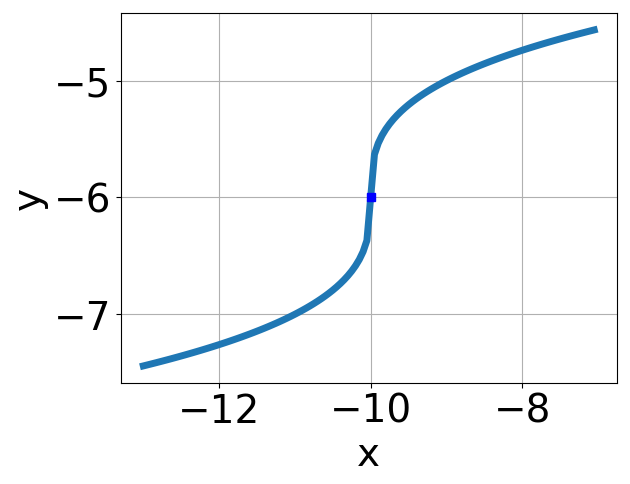
\includegraphics[width = 0.3\textwidth]{../Figures/radicalEquationToGraphAC.png}\item 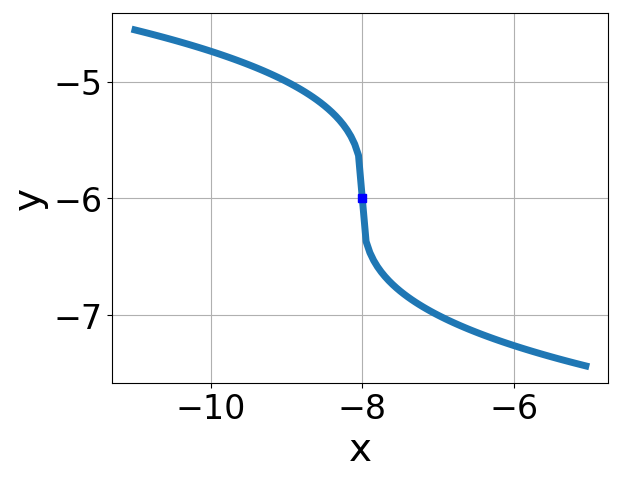
\includegraphics[width = 0.3\textwidth]{../Figures/radicalEquationToGraphBC.png}\item 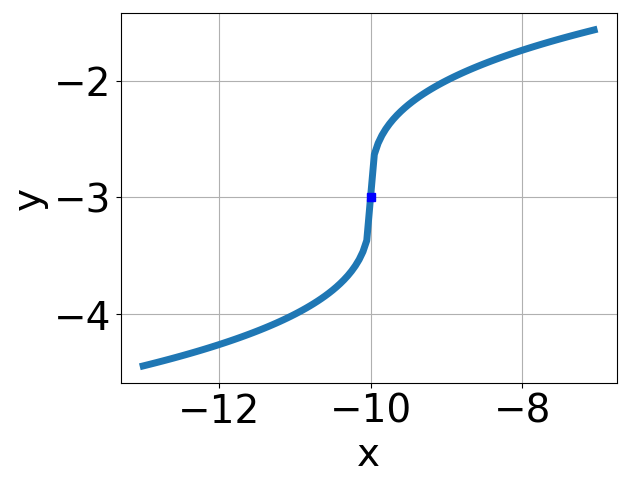
\includegraphics[width = 0.3\textwidth]{../Figures/radicalEquationToGraphCC.png}\item 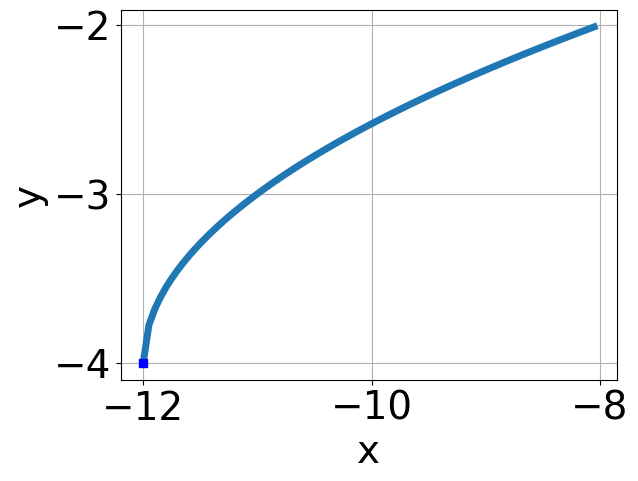
\includegraphics[width = 0.3\textwidth]{../Figures/radicalEquationToGraphDC.png}\end{multicols}\item None of the above.
\end{enumerate} }
\litem{
Choose the equation of the function graphed below.
\begin{center}
    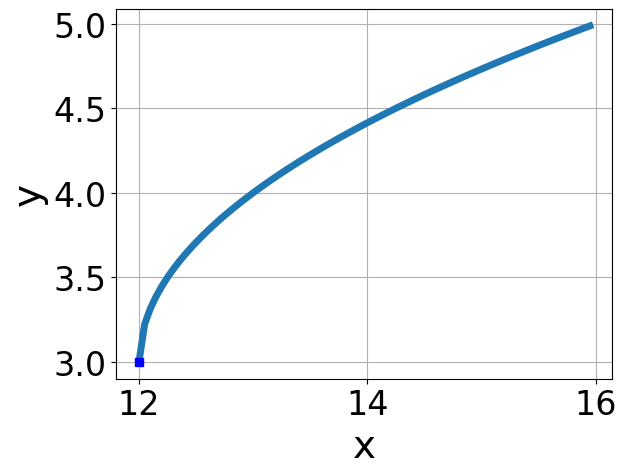
\includegraphics[width=0.5\textwidth]{../Figures/radicalGraphToEquationCopyC.png}
\end{center}
\begin{enumerate}[label=\Alph*.]
\item \( f(x) = - \sqrt[3]{x - 10} - 3 \)
\item \( f(x) = \sqrt[3]{x - 10} - 3 \)
\item \( f(x) = \sqrt[3]{x + 10} - 3 \)
\item \( f(x) = - \sqrt[3]{x + 10} - 3 \)
\item \( \text{None of the above} \)

\end{enumerate} }
\litem{
What is the domain of the function below?\[ f(x) = \sqrt[6]{-9 x + 8} \]\begin{enumerate}[label=\Alph*.]
\item \( [a, \infty), \text{where } a \in [0.96, 1.53] \)
\item \( (-\infty, \infty) \)
\item \( (-\infty, a], \text{ where } a \in [0.63, 1.02] \)
\item \( (-\infty, a], \text{where } a \in [1.05, 1.58] \)
\item \( [a, \infty), \text{where } a \in [0.81, 0.98] \)

\end{enumerate} }
\litem{
Choose the equation of the function graphed below.
\begin{center}
    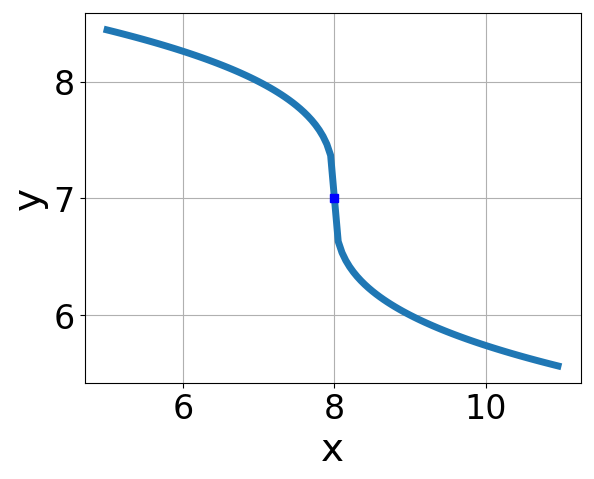
\includegraphics[width=0.5\textwidth]{../Figures/radicalGraphToEquationC.png}
\end{center}
\begin{enumerate}[label=\Alph*.]
\item \( f(x) = - \sqrt{x + 14} + 6 \)
\item \( f(x) = - \sqrt{x - 14} + 6 \)
\item \( f(x) = \sqrt{x + 14} + 6 \)
\item \( f(x) = \sqrt{x - 14} + 6 \)
\item \( \text{None of the above} \)

\end{enumerate} }
\litem{
Solve the radical equation below. Then, choose the interval(s) that the solution(s) belongs to.\[ \sqrt{-21 x^2 - 24} - \sqrt{-54 x} = 0 \]\begin{enumerate}[label=\Alph*.]
\item \( x \in [0.7,3.8] \)
\item \( x \in [-0.5,1.6] \)
\item \( \text{All solutions lead to invalid or complex values in the equation.} \)
\item \( x_1 \in [-1, 0] \text{ and } x_2 \in [-3,1] \)
\item \( x_1 \in [-0.5, 1.6] \text{ and } x_2 \in [-2,8] \)

\end{enumerate} }
\litem{
Choose the graph of the equation below.\[ f(x) = - \sqrt{x - 8} + 3 \]\begin{enumerate}[label=\Alph*.]
\begin{multicols}{2}\item 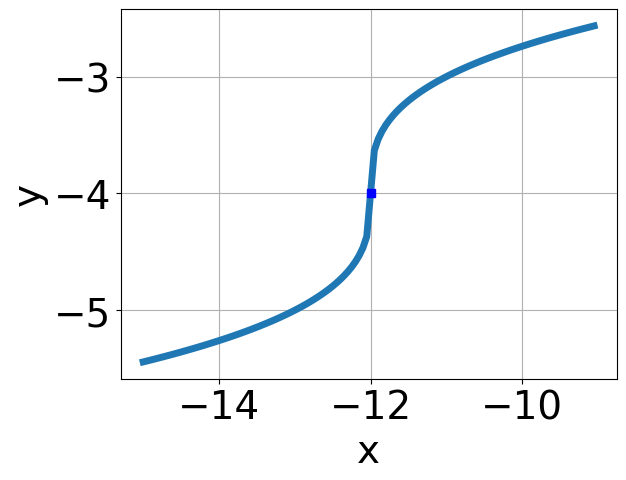
\includegraphics[width = 0.3\textwidth]{../Figures/radicalEquationToGraphCopyAC.png}\item 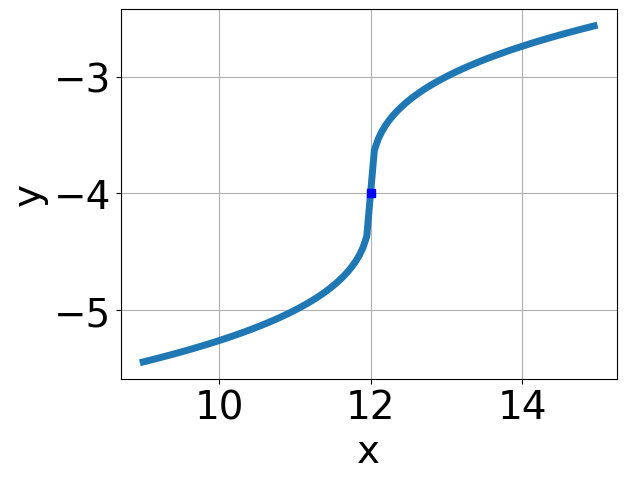
\includegraphics[width = 0.3\textwidth]{../Figures/radicalEquationToGraphCopyBC.png}\item 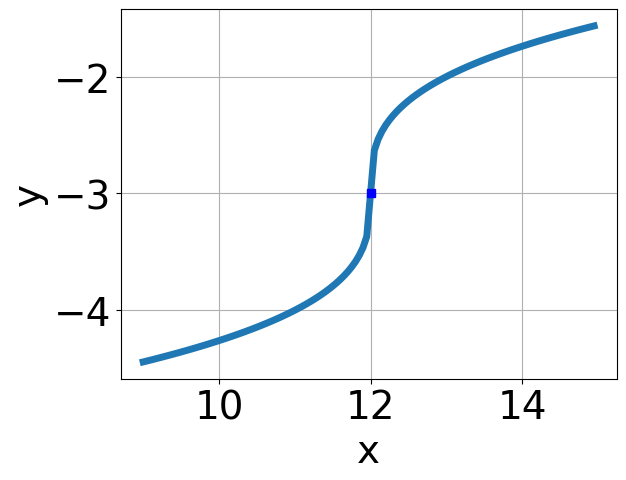
\includegraphics[width = 0.3\textwidth]{../Figures/radicalEquationToGraphCopyCC.png}\item 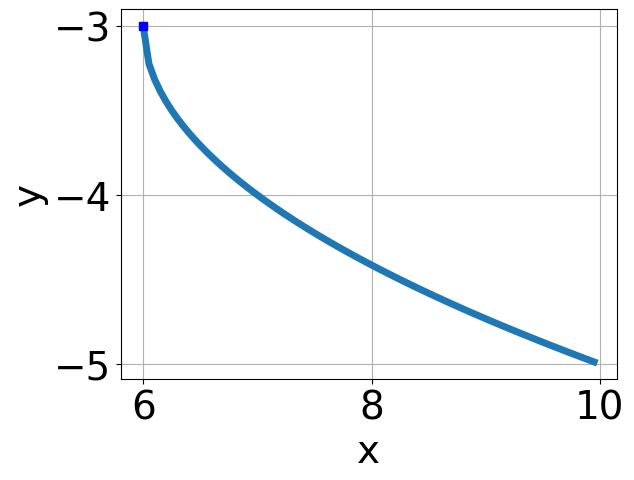
\includegraphics[width = 0.3\textwidth]{../Figures/radicalEquationToGraphCopyDC.png}\end{multicols}\item None of the above.
\end{enumerate} }
\end{enumerate}

\end{document}